\documentclass[a4paper]{article}
\usepackage[pdftex]{graphicx}
\usepackage[utf8]{inputenc}
\usepackage{enumerate}
\usepackage{siunitx}
\sisetup{locale=DE}
\usepackage{icomma}
\usepackage{amssymb}
\usepackage{tikz}
\usepackage{href-ul}
\hypersetup{
	colorlinks=true,
	linkcolor=blue,
	urlcolor=blue}
\usepackage{geometry}
\geometry{a4paper, top=15mm, left=15mm, right=15mm, bottom=15mm,
	headsep=10mm, footskip=12mm}
\hyphenation{weight-force}

\begin{document}
	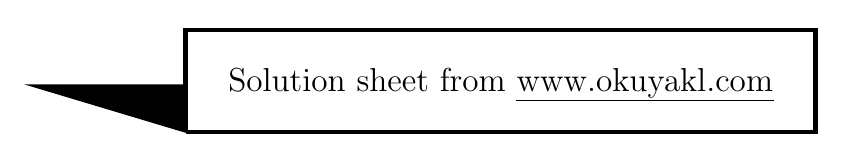
\begin{tikzpicture}(10,3)
		\draw[ultra thick](2,0) --(10,0) -- (10,1.3) --(2,1.3) -- (2,0);
		\draw[fill=black](2,0)-- (0,.6) -- (2,.6) -- (2,0);
		\node at (6,.6) {\large Solution sheet from \href{http://www.okuyakl.com}{www.okuyakl.com}};
	\end{tikzpicture}
	\vspace{0.5 cm}
	
	\noindent{\bf Task 1. a)}\\
	\begin{minipage}{0.7\textwidth}
		The surface of a body is always more or less rough. When two bodies come into contact, these roughnesses interlock with each other, and the higher the contact pressure, the more strongly they become. The circled area in the sketch below represents an enlargement of the contact point.
	\end{minipage}
	\begin{minipage}{0.3\textwidth}
		\includegraphics[width=5 cm]{reib122}
	\end{minipage}
	\vspace{0.5 cm}
	
	\noindent{\bf Task 1. b)}\\
	You can reduce the contact force, smooth the surfaces by polishing or add a lubricant such as oil or soft soap.
	\vspace{0.5 cm}
	
	\noindent{\bf Task 1. c)}\\
	With a one-sided lever, the forces both act on one side of the joint; Examples: nutcracker, fishing rod, golf club.
	\vspace{0.5 cm}
	
	\noindent In a two-sided lever, the joint is between the points of application of the forces; Examples: pliers, scissors, rocker.
	\vspace{0.5 cm}
	
	\noindent{\bf Task 1. d)}\\
	The torque $M$ is the product of the acting force $F$ with its force or lever arm $a$. When a force acts on a lever, it causes a torque. It is larger the larger $F$ and the longer $a$.
	\vspace{0.5 cm}
	
	\noindent
	\begin{minipage}{0.4\textwidth}
		\noindent{\bf Task 2. a)}\\
		\includegraphics[width=6 cm]{efen122}
	\end{minipage}
	\begin{minipage}{0.6\textwidth}
		\noindent{\bf Task 2. b)}\\
		The sliding friction force is proportional to the normal force $F_N$. This follows from the fact that the measuring points lie on a straight line from the origin.
		\vspace{0.5 cm}
		
		\noindent{\bf Task 2. c)}\\
		The following applies to the coefficient of sliding friction $\mu$:
		$$ F_G= \mu \cdot F_N$$
		We choose a pair of values that lie on the line, solve for $\mu$ and insert:
		$$ \mu = {F_G \over F_N}={\SI{0.91}{\newton} \over \SI{3.0}{\newton}}=0.30$$
	\end{minipage}
	\vspace{0.5 cm}
	
	
	\noindent{\bf Task 3.}\\
	There are very many possibilities; you can stack the cuboids or place them one behind the other. The wooden block has the lowest coefficient of friction. So the cheapest option is for the wooden cuboid to lie on the bottom and support the other two cuboids. Then the weights are only multiplied by the smallest $\mu$.
	\vspace{0.5 cm}
	
	\begin{minipage}{0.5\textwidth}
		\noindent{\bf Task 4.}\\
		The lifting work is
		$$W=F_G\cdot h \quad \Rightarrow \quad h = {W \over F_G} = {\SI{12000}{\joule} \over \SI{1500}{\newton}} = \SI{8 }{\meter}$$
		
		
		\noindent{\bf Task 5.}\\
		Work is power times time and at the same time (frictional) force times distance:
		$$ P \cdot t = \mu \cdot F_G \cdot s \quad \Rightarrow \quad F_G = {P \cdot t \over \mu \cdot s}=
		{\SI{20}{\watt} \cdot \SI{10}{\second} \over 0.20 \cdot \SI{2.0}{\meter}} = \SI{500}{\newton} $$
		Unit check:
		$$ {\SI{}{\watt}\cdot \SI{}{\second} \over \SI{}{\meter}}= {\SI{}{\newton\meter} \over \SI{} {\meter}}=\SI{}{\newton}$$
	
	\end{minipage}
	\hfill
	\begin{minipage}{0.5\textwidth}
			\begin{center}
			\includegraphics[width=7 cm]{../../viecher/eendcomic.pdf}
			
			Here you can go back to the \href{https://www.okuyakl.de/phys/p8reibL122/ae122.pdf}{task sheet}
		\end{center}
		
	\end{minipage}
	

\end{document}